%\documentclass[11pt]{article}

%\usepackage{graphicx}
%\usepackage{amssymb}
%\usepackage{amsmath}
%\usepackage[margin=2.5cm]{geometry}

%\usepackage[round]{natbib}
%\usepackage[colorlinks=true,citecolor=blue]{hyperref}
%\usepackage{hypernat}

%\bibliographystyle{plainnat}

\chapter{Literature Review} \label{chap:litreview}

%\title{Literature Review}
%\author{Peter Ashwell}
%\date{}

%\begin{document}
%	\maketitle

\subsection{Distance Measures for Time Series}
	\label{sec:distancemeasures}
	
	\subsubsection{Introduction}
	The most primitive approach to analysing a time series is to overlay it onto another time series with known class and see how well it fits by calculating the Euclidean \emph{distance} between the two curves. A low distance indicates a high similarity. By comparing the test curve to a number of training samples the most likely class is determined as that having the lowest distance (or lowest distance below some threshold). This approach, called a \emph{Nearest Neighbour} classification, can be very effective if the time series are uniform within their class. 
	\paragraph{}
	Unfortunately, astronomical time series do not have that property. Although they have the same form in terms of peaks, throughs, plateaus, lines, wobbles and so on, the actual magnitude and time over which astronomical transients unfold is not necessarily the same. These issues are called amplitude scaling and time warping. These two distortions, compounded with the lack of complete data make Euclidean distance useless. 
	\paragraph{}
	Overcoming this distance measure issue may yield in itself a solution to our problem. Additionally, distance measures are likely to be integral to data preprocessing or to the application of other approaches such as temporal grammars, support vector machines and shapelets discussed later. The following section is devoted to an exploration of more flexible distance measures than the Euclidean distance.
	
	\subsubsection{Dynamic Time Warping}
	Dynamic Time Warping (DTW) is a technique first introduced in \citep{sakoe1978dynamic} and was popularised in \citep{berndt1994using} with successful application to speech signal classification. The algorithm is a dynamic programming approach to that allows the matching to `skip' parts of either time series in order to align them better. The distance of two time series under DTW is then the minimum across all possible matchings. Figure ~\ref{fig:dtwinaction} shows dynamic time warping finding a better alignment for two sequences than Euclidean distance. Dynamic time warping deals very well with changes in the way transients unfold but is not guaranteed to find a good match in the presence of amplitude scaling. It also seems hard to extend this algorithm to matching subsequences as required by our problem.
	\paragraph{}
	Should dynamic time warping or some modification be found useful to us, an extension of the computation that allows on-line updating would be very attractive for dealing with the \textbf{real-time} complication. Such an extension is given in \citep{capitani2007warping}, which gives an algorithm with constant time updating of DTW distance for a time series stream. The distance measure so produced is a close approximation of the full DTW distance.
	
	\begin{figure}[h!]
			\label{fig:dtwinaction}
	\centering
	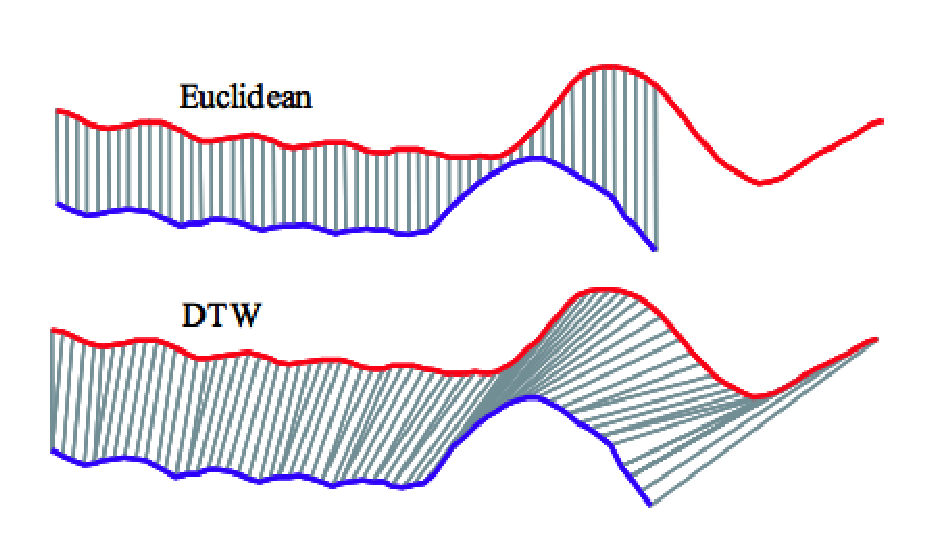
\includegraphics[width=100mm]{/Users/peter/honors/thesis/litreview/images/dtw.eps}
	\caption{Dynamic time warping finding a superior alignment for two time series than Euclidean distance. Alignment is indicated where a grey line joins two points of the series.}
	\end{figure}
	%Still RODO: \citep{berndt1994using}, \citep{keogh2001derivative}

	\subsection{Longest Common Subsequence for Time Series}
	A similar distance measure to DTW is the Longest Common SubSequence (LCSS). LCSS differs from DTW mainly in that all components of both series do not need to be included in the matching. The most similar components of each series are compared in the distance measure only. This approach will find be able to match subsequences to series and cope with time warping at the same time. In \citep{vlachos2002discovering}, an implementation of LCSS that allows translations (not scaling) in space and is fast to compute is given. The translations are incorporated into the dynamic programming algorithm as another dimension to search through.  In the paper it is applied to accurately recognise human gestures presented as multivariable time series in the presence of time warping and translations in space.
	\paragraph{}
	It is possible that this algorithm could be modified to work over different amplitude scalings as well, solving three of our difficult distance complications at once. Such a modification would likely incur additional computational expense. 
	
	\begin{figure}[h!]
	\centering
	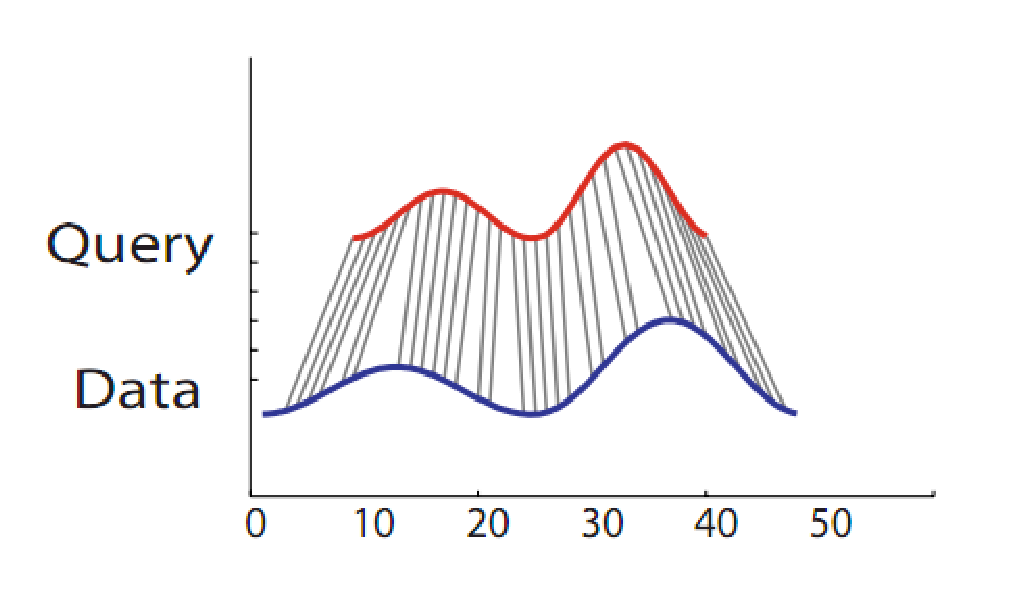
\includegraphics[width=100mm]{/Users/peter/honors/thesis/litreview/images/lcss.eps}
	\label{fig:lcss}
	\caption{Longest Common Subsequence Distance match between a test (query) curve and a training sample (data)}
	\end{figure}
	% TODO something on uniform scaling measures \citep{fu2005scaling}
	
	\subsubsection{Complexity distance} 
	An interesting recent paper of note is \citep{batista2011complexity}. This paper attempts to produce a distance measure based on the abstract notion of complexity, the relative smoothness or bumpiness of a curve. A simple approach to this suggested in the paper is to factor into an existing distance measure (for example, euclidean distance) the relative length of the two time series. For example, if $A$ and $B$ are two time series, C(A) and C(B) are the lengths of $A$ and $B$, and E(A, B) is their euclidean distance, then a new distance measure would be:
	\begin{center}a
	\begin{equation*}
		D(A,B) = \frac{\max(C(A), C(B))}{\min(C(A), C(B))}E(A,B)
	\end{equation*}
	\end{center}
	 The intuition here is that the length of the time series roughly corresponds to its variance over time - the closer two curves are in length the closer they are in complexity. The paper gives good results for a complex time series representing leaf outlines. A similar idea may help to improve classification accuracy for astronomical time series.
	
	\subsection{Gaussian Processes for regression and smoothing of time series}
	\subsubsection{Introduction to Gaussian Processes (GPs)}
	A Gaussian Process (GP) is a statistical model of data that can be used for regression, noise-filtering, classification and prediction. In this section a discussion of the regression and noise-filtering abilities will be presented in the hopes of addressing the \textbf{distortions} issue. A thorough introduction and exploration of gaussian processes can be found in \citep{rasmussen2006gpfml}. A brief overview for the purposes of discussion is provided here.
	
	\paragraph{}
	A GP consists of a multivariate gaussian distribution, where each dimension of the distribution corresponds to an index (in this case, time index) of an input point, say $x$. Gaussian distributions are defined by a mean and a covariance matrix. GPs are more general in that the entries of the covariance matrix are determined by a covariance function $k$. 
	\begin{figure}[ht!]
	\centering
	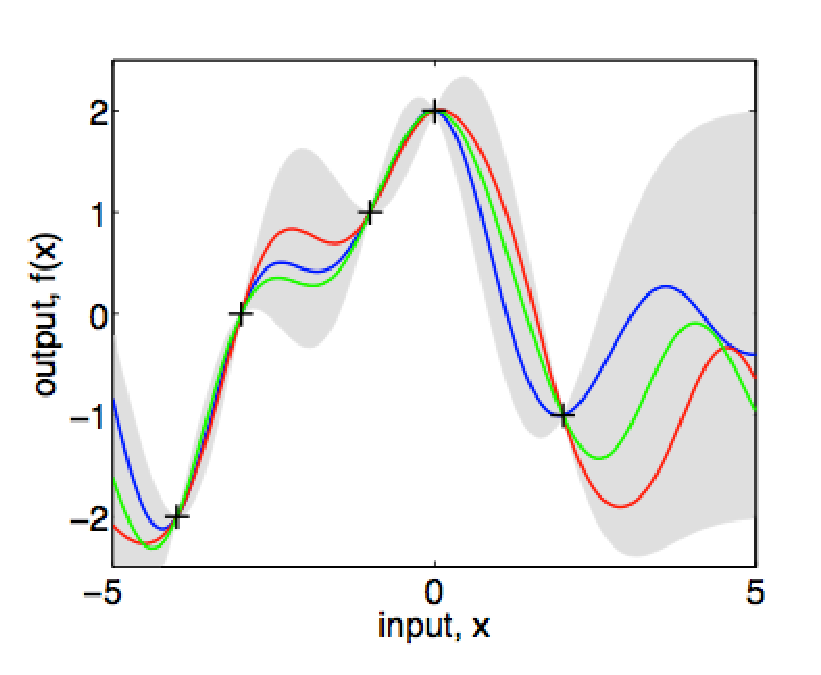
\includegraphics[width=100mm]{/Users/peter/honors/thesis/litreview/images/gpregression.eps}
	\label{fig:gaussianprocessregression}
	\caption{A Gaussian Processes doing Non-Linear Regression on a Time Series. The crosses indicate observations, while the grey bands indicate uncertainty. Some possible underlying functions drawn from processes are shown in green, blue and red}
	\end{figure}
		An evaluation of GPs for regression is carried out in \citep{rasmussen1996evaluation}, demonstrating that GPs are competitive with neural networks on non-linear regression tasks, even performing slightly better when large amounts of noise are present.
%	\begin{center}
%	\begin{align*}
%		\mathcal{GP}(m(\mathbf{x}), k(\mathbf{x}, \mathbf{x}^{\prime})) \\
%	\end{align*}
%	\end{center}
	\paragraph{}
	Covariance functions determine the influence that the points in the distribution have on each other. They are used to control the amount of flexibility and smoothness in the function that the distribution represents. This is done both through the choice of function (popular choices are the squared exponential or the matern functions), and \emph{hyperparameters} to the chosen function. Some commonly used hyperparameters are lengthscale, noise variance and signal variance These correspond respectively to the expected influence of points based on their distance apart in the index, the expected fluctuation in height and expected noise in the data. Optimising the hyperparameters for the dataset is key to getting good regression, prediction and noise filtering.

	\begin{figure}[ht!]
	\centering
	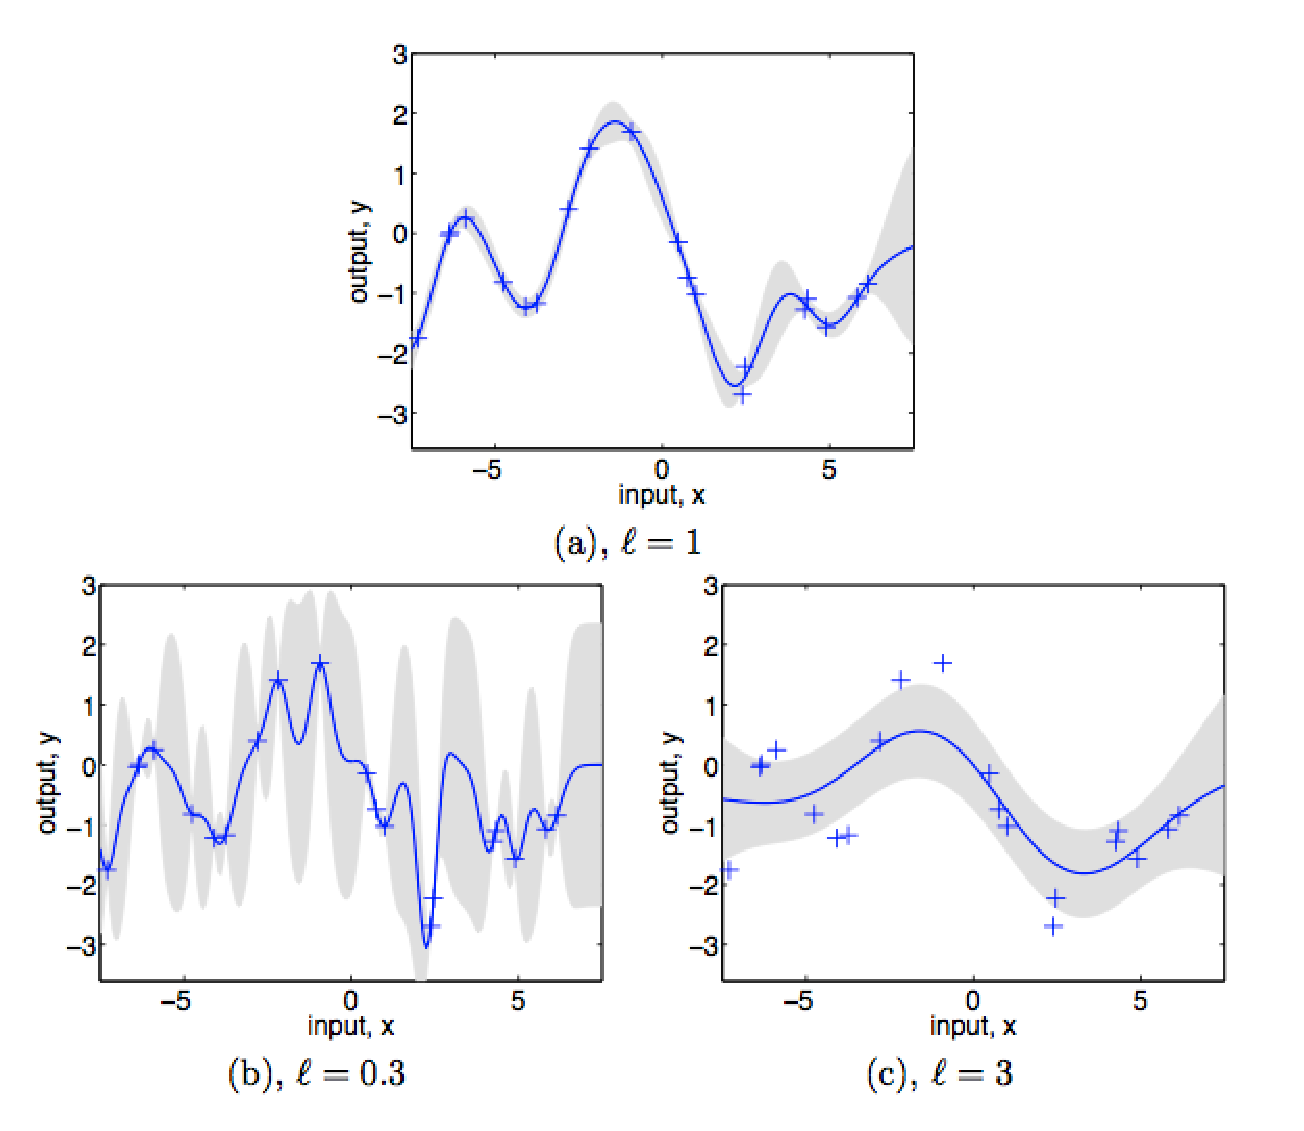
\includegraphics[width=140mm]{/Users/peter/honors/thesis/litreview/images/covariance.eps}
	\caption{3 Gaussian Process interpretations of the same data with varying lengthscales ($l$). The variance bands of the three plots demonstrate that choosing the right hyperparameters is important for accurate regression.}
	\label{gaussianprocesshyperparameters}
	\end{figure}
	

	
	\subsubsection{Sparse Gaussian Processes}
	The time and space complexity of the fundamental GPs is prohibitive for large volumes of data. In recent years several versions of GPs with approximations to covariance functions have been developed to cope with these constraints. These improvements give a time complexity of $O(mn)$ for training time and $O(m^{2})$ for prediction where m is the number of basis functions and $m << n$. The most recent versions of sparse GPs are Sparse Spectrum Gaussian Processes (SSGPs) in \citep{rasmussen2010ssgpr} which use periodic basis functions in the approximation. Sparse Multiscale GPs \citep{walder2008sparse} and Fully Independent Training Conditional (FITC) \citep{snelson2005sgppi} comprise the state of the art. Despite a sensitivity to overfitting on one highly non-linear dataset, SSGP otherwise outperforms FITC and SPGP. With the excepting of the overfitted dataset, all implementations approach the error of a full GP as the number of basis functions ($m$) in the approximation is sufficiently large.

	\subsubsection{On-line Gaussian Processes}
	Standard GPs can be altered to allow for on-line updates of the training variables, see \citep{osborne2007gaussian}. Recently, sparse models have also been implemented that also allow for fast on-line updating. In \citep{ranganathan2011online}, a sparse GP is presented giving an $O(n)$ update time per addition of an additional point. These GPs have full predictive power and outperform state-of-the-art sparse GPs on non-linear data sets. There are limitations on this algorithm however, most importantly that optimising the hyperparameters to new data is a costly $O(n^{2})$ step. This is not ideal since we do not know anything about the structure of our unfolding time series and some tuning is necessary for good results. However, if this issue can be overcome, these are an attractive option for solving the \textbf{distortions} problem.

	\subsection{Summary of Distortion Handling Methods}
	LCSS is the most promising distance measure proposed and may possibly solve our warping and amplitude scaling distance measure problems, whilst also working for subsequence queries as the problem demands. Gaussian Processes seems like a promising solution to missing and noisy data, but whether the sparse, on-line version is suitable for our problem will need to be tested. In all, these are ideas that could potentially remedy all of our \textbf{distortion} complications.
	
	\subsection{Approaches to Time Series Classification}
	This section gives a general discussion of techniques developed for analysing and classifying time series. Some of the methods will be more useful as \emph{features} for generic machine learners. Falling under this category are wavelets, temporal grammars and periodograms. Others are more directly useful for classification, such as shapelets, support vector machines (SVMs), and phase invariant kernels. Each subsection will aim to discuss the technique in terms of the relevant complications in our problem, namely the \textbf{real-time}, \textbf{precision} and \textbf{periodic} issues. Not all the methods discussed here are appropriate for streams but some modifications or extensions of them could be. A discussion of particular approaches to stream classification is given in section~\ref{sec:timeseriesstreams}.
	
%	TODO a paragraph on feature extraction
%	A lot of the methods discussed so far are explicit analysis tools that deal with some particular kind of time series and have varying strengths and weaknesses depending on what is being classified, for example, Fourier transforms for periodic time series. These independent strengths can be leveraged with feature extraction to produce a very powerful and general classifier. 

%	\subsection{Statistical Approaches}
%	\begin{itemize}
%		\item Autoregressive moving average models
%		\item Bayesian Models
%	\end{itemize}
	
	\subsection{Frequency Domain Approaches}
	\subsubsection{Introduction}
	Frequency domain analysis is the most well explored technique for studying astronomical time series. In itself it is highly effective for identification and classification of periodic stars - one category of astronomical time series our system needs to deal with. Additionally, the outputs of the various techniques can be used to extract features for time series without periodic structures. These features can then be used in generic feature based machine learning classifiers. Worth noting is that frequency metrics are less sensitive to noise and time warping than time domain analysis. A brief survey of the techniques and how they may be applied to our problem follows.
	\subsubsection{Discrete Fourier Transforms and the Lomb-Scargle Periodogram}
	A Fourier transformation is decomposition of a continuous function into sinusoids. The strength of the peak for each component of the decomposition indicates the strength of that component in the original signal. 
	\begin{figure}[ht!]
	\centering
	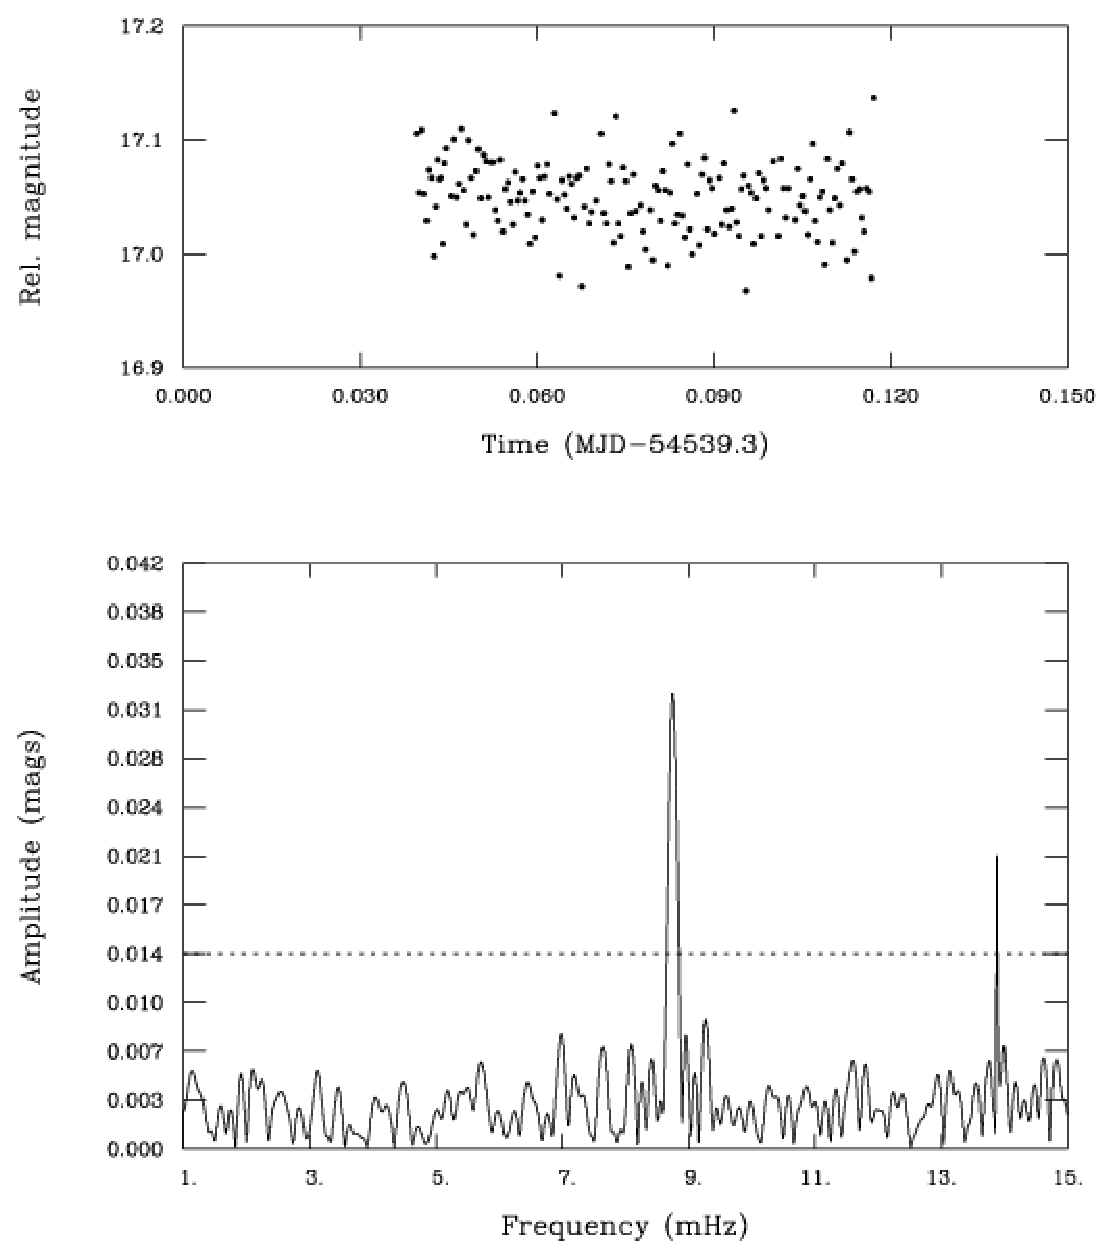
\includegraphics[width=110mm]{/Users/peter/honors/thesis/litreview/images/discretefft.eps}
	\label{fig:fouriertransform}
	\caption{Fourier Transform of an astronomical time series. The peaks represent the most significant periodic components. In this case the signal has two clear periodicities.}
	\end{figure}
	There is a version of the Fourier transform that works for discrete data such as ours, but unfortunately is sensitive to discontinous regions. The Lomb Scargle Periodogram, introduced in \citep{lomb1976least} and \citep{scargle1982studies}, is a spectral decomposition that copes with this issue. The method involves fitting a number of sinusoidal basis functions onto a dataset using least squares regression. The output is a spectral decomposition of weighted sinusoids like the Fourier transform.
	
	%\paragraph{}
	%A periodogram construction can be used to detect if a signal is periodic or not as outlined in: \citep{cincotta1995astronomical}

	\subsubsection{Wavelets}
	A wavelet decomposition for a time series is a transformation into a number of basis waveforms. The Fourier transformation presented above is one such decomposition, but many other forms exist with useful properties such as the Haar wavelet transform. 
	\paragraph{}
	The Haar wavelet decomposition produces a set weighted component rectangular shaped waves of decreasing granularity. The output of this process on a time series is given in \ref{fig:haarreconstruction}.

	\begin{figure}[ht!]
	\centering
	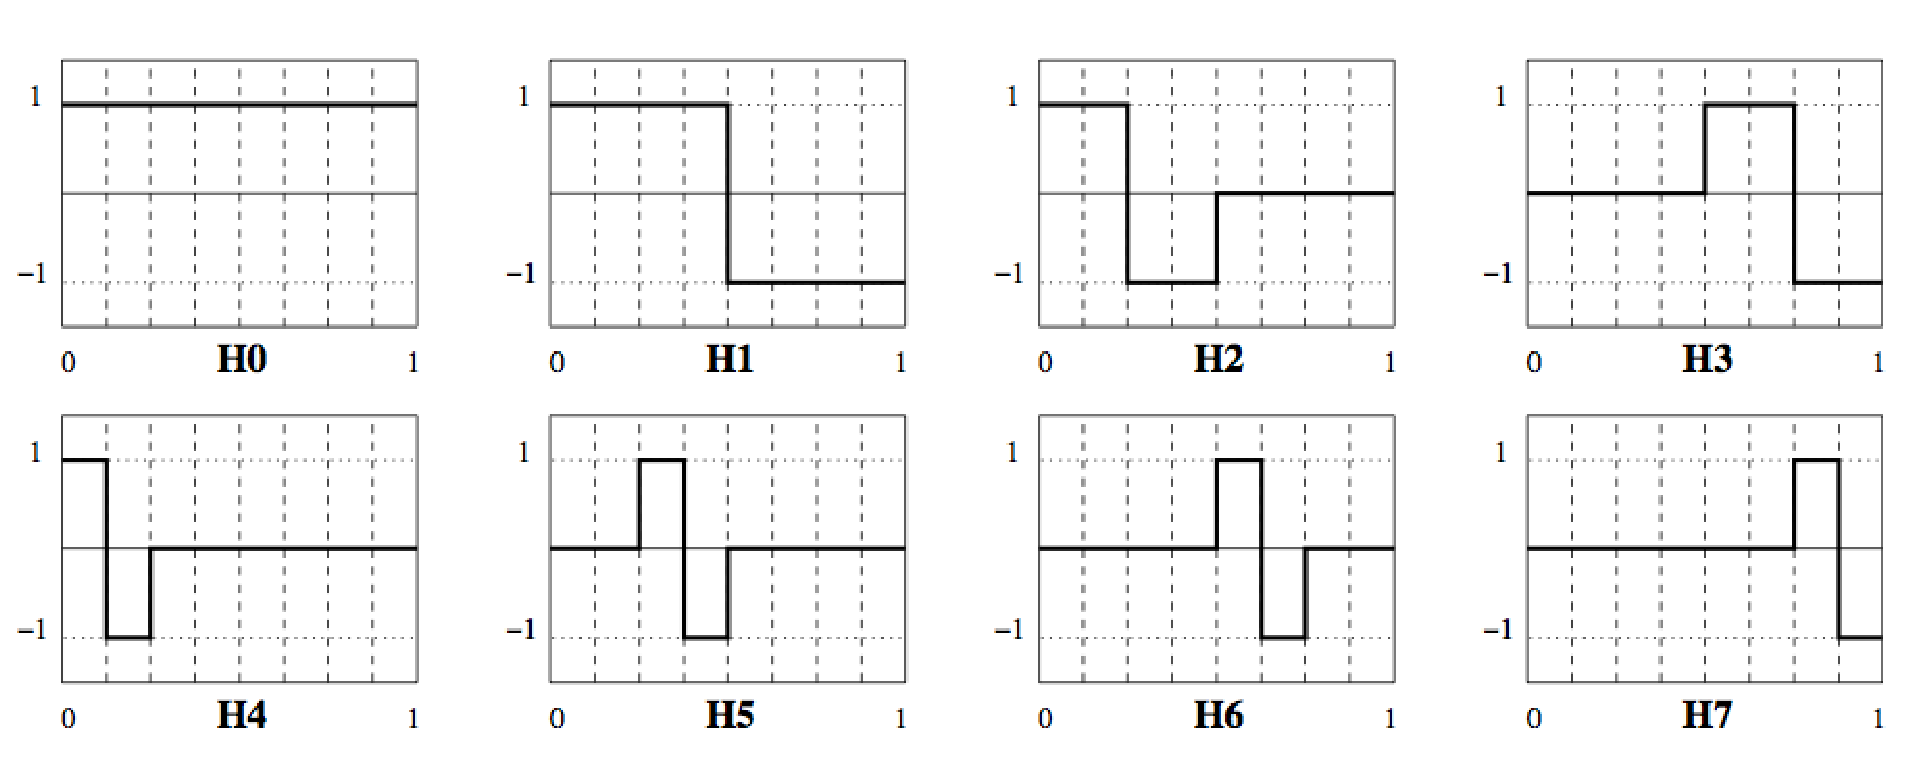
\includegraphics[width=120mm]{/Users/peter/honors/thesis/litreview/images/haarbasis.eps}
	\caption{The first 8 Haar basis wavelets.}
	\label{fig:haarwavelets}
	\end{figure}
	
	\begin{figure}[ht!]
	\centering
	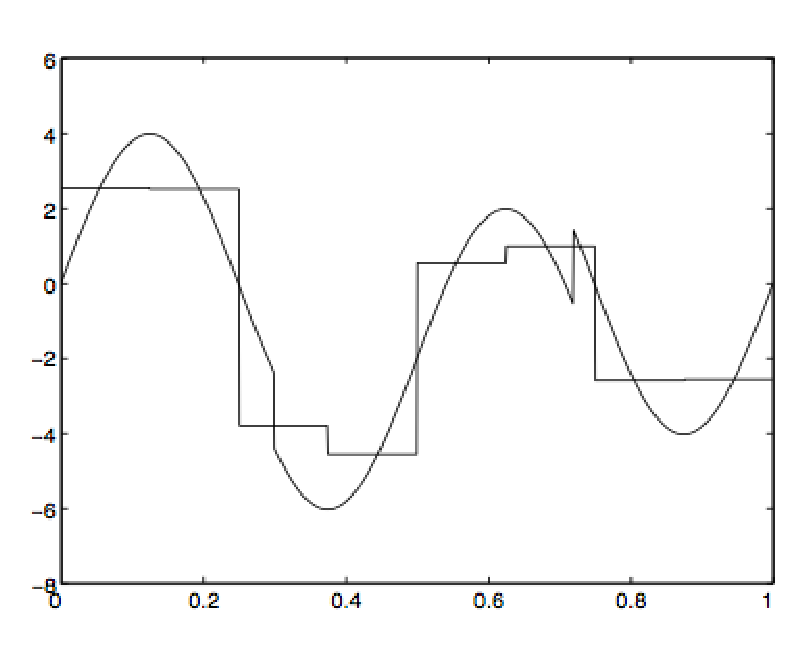
\includegraphics[width=80mm]{/Users/peter/honors/thesis/litreview/images/haarreconstruction.eps}
	\caption{A time series reconstructed from its Haar wavelet decomposition.}
	\label{fig:haarreconstruction}
	\end{figure}


	Haar wavelets as a representation of a time series bear some similarity the local patterns extracted in \ref{sec:timeseriesstreams}. This transformation takes linear time in the length of the time series. As explored in \citep{popivanov2002similarity}, The structure of the rectangular Haar wavelet makes similarity comparison for time series very fast, an appealing property for the large data volumes involved in this research. Unfortunately, Haar Wavelets are still inflexible under astronomical time series \textbf{distortions}, but could possibly be utilised for similarity search with a non-Euclidean distance measure.
	
	% TODO add this>
	%\citep{price2011haar}
	%\citep{zhang2005blind}
	%\citep{zhang2006feature}
	%\citep{popivanov2002similarity}
	%\citep{mondal2010wavelet}
	
	\subsubsection{Phase Invarant Kernels}
	Besides spectrum analysis, an approach to classifying periodic stars is to use a phase-invariant distance measure. Phase invariant means that no matter what translation the time index is under, the distance between the two light curves is the same.
	\paragraph{}
	In \citep{wachman2009kernels} a phase invariant Kernel is proposed for periodic astronomical time series. It is immediately suitable for the nearest neighbour algorithm. The first proposed kernel is computed for two time series $x$ and $y$ as:
	\begin{center}
	\begin{equation*}
		K(x,y) = \sum\limits_{i=1}^{n}e^{ x \cdot y_{+i}}
	\end{equation*}
	\end{center}
	That is, the exponential of the dot products for all possible discrete alignments of the two time series. 	This measure gives much higher scores to those time series for which there exists some very close alignment.
	\paragraph{}
	More interestingly, with some modification this kernel is also suitable for use in a support vector machine. With this approach the authors get excellent results a dataset of real light curves with accuracies of greater than 99\%. The kernel score is fast to compute with a computational bound of $O(n\log n)$. The authors do not address the issue of amplitude scaling and classify with full light curves, so there are still some complications for our problem that this approach does not cover. Nevertheless, the use of handcrafted kernels for time series is an interesting one, explored further in Section \ref{sec:svms}.
	
	\subsection{Time Domain Analysis Approaches}
	Time series analysis which works directly with the time indexed data is called \emph{time domain} analysis. The simplest possible classification method, nearest neighbour classification, was already mentioned in Section~\ref{sec:distancemeasures} when discussing distance measures for time series. Wavelets and shapelets can be used as features for generic learners such as support vector machines and neural networks. Additionally, those same machine learners can be applied directly to the data for classification.

	\subsubsection{Shapelets}
	The idea of shapelets, first presented in \citep{ye2009time}, is to find motifs in time series that are maximally discriminative amongst the classes of training examples. Once these motifs are extracted, any distance measure can be used to apply the motifs from the various classes to a test case. The training class with the lowest scoring motif is chosen as the label.
	\begin{figure}[ht!]
	\centering
	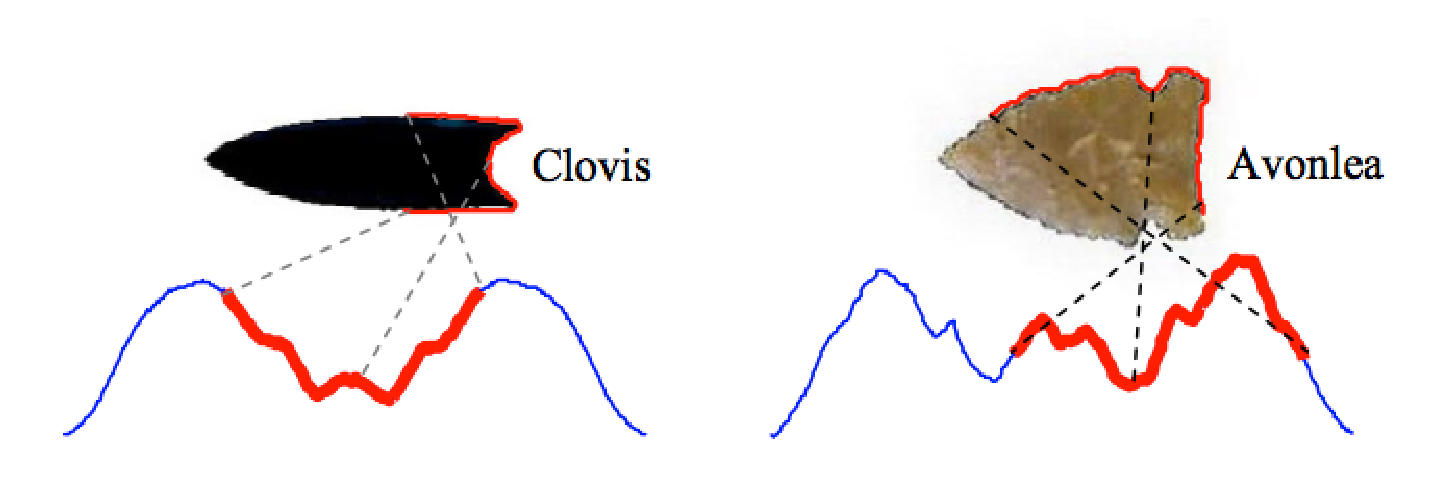
\includegraphics[width=120mm]{/Users/peter/honors/thesis/litreview/images/shapelet.eps}
	\caption{Two time series representing arrowhead shapes with representative shapelets highlighted in red.}
	\label{fig:shapelets}
	\end{figure}
	The authors in the paper propose an information gain approach to choosing which shapelets to represent each class in a decision tree structure - only those shapelets which produce the fastest separation of the training classes are used. This approach is appealing because it allows fast classification that should also be more resistant to distortions than classification than attempts to compare entire time series. An extension of shapelets to classifying time series streams is given in Section~\ref{sec:timeseriesstreams}.

	\subsubsection{Support Vector Machines}
	\label{sec:svms}
	Support Vector Machines are machine learning tools that work by computing a so-called maximum margin that separates two classes in a feature space. A simple example of a support vector machine working in euclidean space is presented below. Multi class classification is possible by feeding a test case into an ensemble of binary classifiers, facing them off against each other in a tournament style. The winner of the tournament is chosen as the classification for that test case.
	\begin{figure}[ht!]
	\centering
	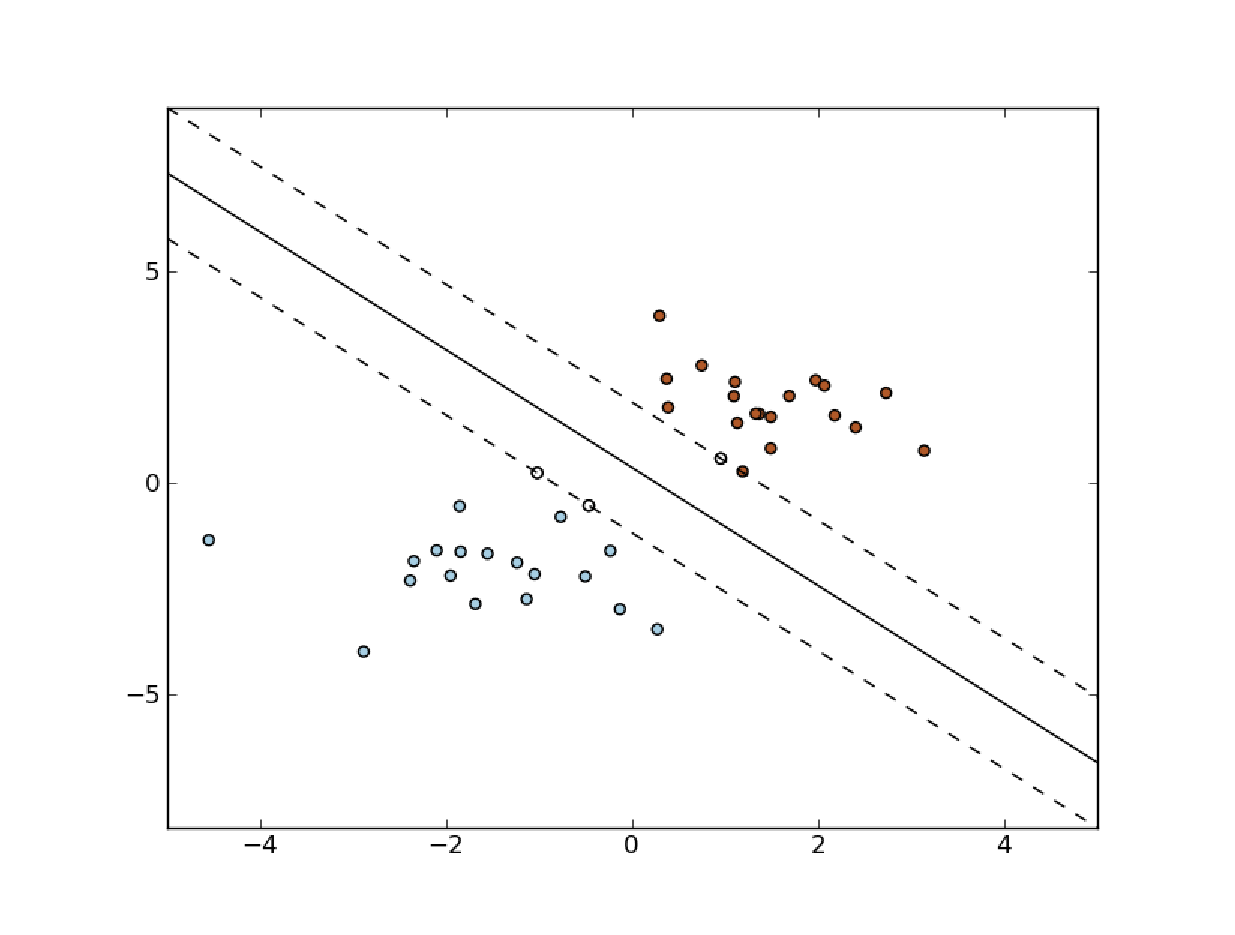
\includegraphics[width=120mm]{/Users/peter/honors/thesis/litreview/images/svmmargin.eps}
	\label{svmtrain}
	\caption{Separation margin for two classes (blue and red dots) produced  by a support vector machine}
	\end{figure}
	\paragraph{}
	A simple suggestion to use one of these SVM ensembles in our task would be to represent a time series with n time indices as a vector in $n$ dimensional Euclidean space. A test class would be fed into the ensemble and whichever time series class it most closely resembles in Euclidean distance would be chosen as the label. Of course, this approach has all the problems that the Euclidean distance measure has as outlined in \ref{sec:distancemeasures}, But classification would be faster (and possibly more accurate) than the nearest neighbour algorithm.
	\paragraph{}
	A modification of the SVM algorithm that is very relevant to our task is outlined in \citep{shimodaira2002dynamic} and \citep{bahlmann2002online}. In this paper a kernel is developed which uses the dynamic time warping distance of two time series. Kernels can be used to transform time series into points in a new feature space. The SVM algorithm can modified to separate these points if the kernel has certain properties. The proposed kernel unfortunately is not completely suitable (it is not positive semidefinite) and cannot be expected to work properly, but it nevertheless gives comparable performance to Hidden Markov Models on speech and handwriting classification datasets in these two papers. This notion of a kernel designed explicitly to have the distance measure properties we need for our time series is worth exploring further.
	
	%TODO hidden markov models
	%TODO neural networks
	%TODO piecewise approximations
	
	\subsection{Temporal Grammars}
	\subsubsection{Introduction}
	Astronomical time series have forms which make them distinct from each other and from background noise. Peaks, grades of slopes, valleys, bumps and other local features characterise each class. Humans are good at discerning these forms, but to train a machine learning classifier requires some kind of language to express the substructures - a temporal grammar. This Section discusses feature extraction methods for temporal grammars that are both robust for classification and are human interpretable - they can be easily adjusted and reapplied. There are limitations to this technique for our problem in that any features extracted must be invariant to the in-class distortions of astronomical time series. This may be possible if the features are sufficiently abstract.
	\subsubsection{Early Temporal Grammars and Basic Approach}
	Early work in this area consists of approximating a pattern using simple shapes, for example, straight line segments as in as in \citep{keogh1998enhanced}. One attempt at a generalisation of temporal grammars is found in \citep{olszewski2001generalized}, and this is a good introduction to the end-to-end approach. This paper utilises a grammar of \{constant, straight, triangular, trapezoid, sinusoid, exponential\} to the task of pattern representation. This approach is very similar to the shapelet approach except that these features are more abstract, allowing potentially for modifications that cope with stretching and scaling more easily than shapelets. Additionally, the simplified nature of grammar components means that comparing features amongst time series is much faster. 
	\begin{figure}[ht!]
	\centering
	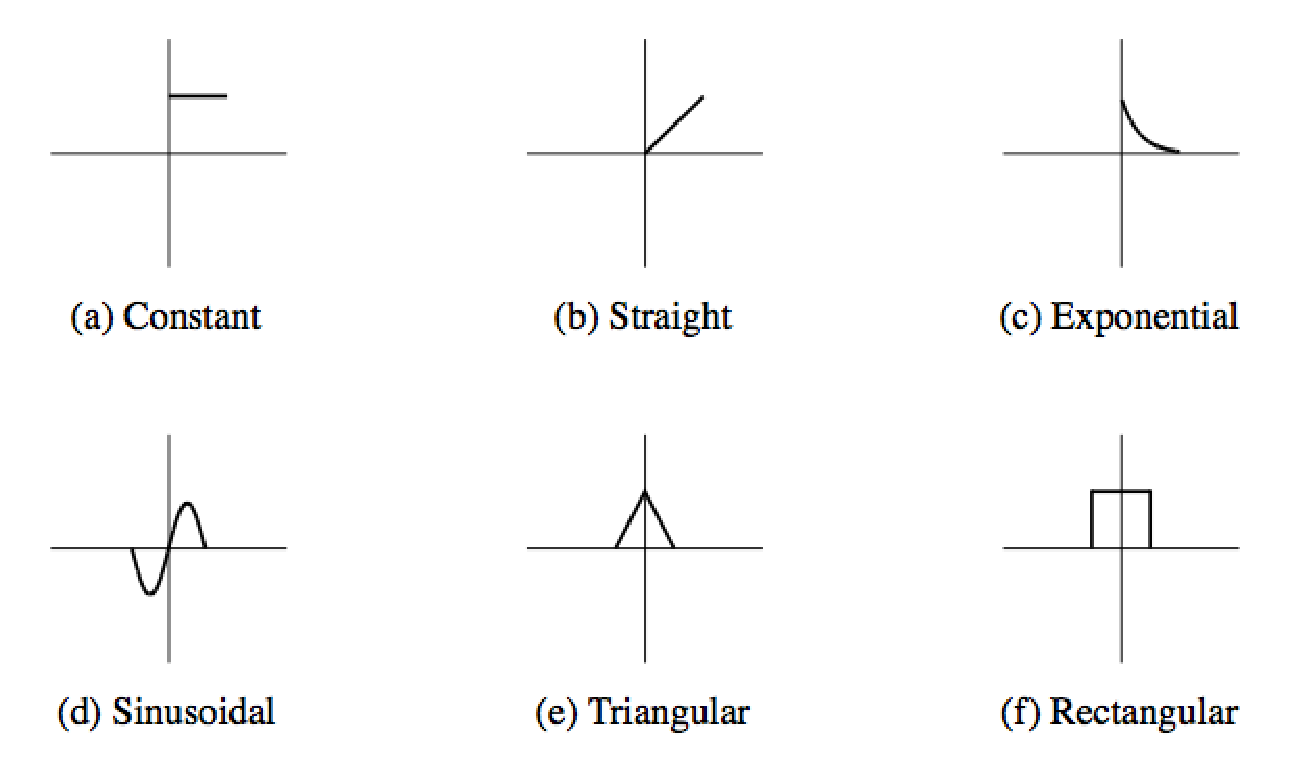
\includegraphics[width=120mm]{/Users/peter/honors/thesis/litreview/images/ozlewskigrammar.eps}
	\caption{Components of temporal grammars used in the Olszewski paper}
	\label{oslewskigrammar}
	\end{figure}
	
	\paragraph{}
	Dynamic programming is used to decide on optimal partitions of the pattern by finding the minimal error choices of substructure pieces. These substructures are then represented as numerical feature vectors which are fed into a standard machine learning classifier. The implementation was run on complex non-linear time series datasets including ECG (Electrocardiogram) data. 
	\paragraph{}
	The paper implements and trials a feature extractor, comparing it with feature extraction methods based on wavelets and fourier transforms. The temporal grammar approach was competitive, and better in many cases. Unfortunately, extraction of these features is a slow process and this approach will unlikely be feasible for time series data streams.
	
	\subsubsection{Recent Improvements and Distortion-Invariant Forms}
	In \citep{kadous2005classification} a more abstract temporal grammar is proposed. In this case, not based on parameterised curve fitting but on more general pattern substructures including plateaus, increasing and decreasing sections and local maxima and minima. The grammar can be extended but it already quite powerful with those features alone. A classifier is built by constructing a decision tree from features extracted from training samples.
	\paragraph{}
	The Kadous temporal grammar is applied to similar datasets as in Olszewski: Etime series and a temporal representation of sign language expressions.  Both datasets are highly nonlinear. Accuracy around the average for professional cardiologists is achieved, notably without any expert background knowledge introduced into the model. The model also outperforms a Hidden Markov Model implementation slightly, with the added bonus that the rules produced are human interpretable (HMM training states are not). 
	\paragraph{}
	Since the features are more abstract than the parameterised curves of the previous section, proposals for dealing with amplitude scaling and warping seem feasible. For an example, one could look at the distributions of local maxima and minima to find likely matches, then search for constant factor differences in their amplitude for confirmation, similarly for plateau length and height. If an algorithm for rapid extraction of features from time series streams were developed, a similar approach could be used in solving this problem.
	
%	Todo talk about papers
%	\begin{itemize}
%	\item Wavelet features for time series stream classification \citep{xing2011extracting}
%	\item Constructing high dimensional feature space for time series classification \citep{eruhimov2007constructing}
%
%	\item Generalized feature extraction for structural pattern recognition in time series data \citep{olszewski2001generalized}
%	\item Classificaiton of Multivariate Time series and Structure Data using Constructive Induction \citep{kadous2005classification}
%	\item Feature Subset Selection and Feature Ranking for Multivariate Time Series \citep{yoon2005feature}
%	\item Efficient Mining of Understanding Patterns from Multivariate Time Series \citep{morchen2007efficient}
%	\item Mining Sequence Classifiers for Early Prediction \citep{xing2008mining}
%	\item Pattern Extraction for Time Series Classification ACTUALLY TIME DOMAIN --- \citep{geurts2001pattern}
%	\item Time series classification based on qualitative space fragmentation \citep{jagnjic2009time}
%	\item Support Vector Machines of interval based features for time series classification \citep{rodriguez2005support}
%	\end{itemize}

	\subsection{Analysis of time series streams}
	\label{sec:timeseriesstreams}
	
	\subsection{Extracting Shapelets and Local Patterns From Streams}
	Several papers propose extensions shape-based feature extraction to streaming time series. One such paper is \citep{chen2007spade}, which presents an algorithm that is supposedly robust to amplitude scaling \emph{and} time warping together, an attractive combination for coping with our \textbf{distortions} problem. The algorithm builds upon existing similar approaches that do not cope well with distortions like \citep{wu2004online}. Local pattern profiles are built from a collection of training curves and bear a strong resemblance to temporal grammars. There may be many overlapping local patterns in a profile - the paper also proposes an algorithm for pruning less descriptive ones.
	\paragraph{}
	The distance measure is calculated by a dynamic programming algorithm based on local pattern comparison between the query time series and the training profiles. The local patterns can be stretched and scaled in the operation of this algorithm - the most important component of the distance measure is that the \emph{shapes} are similar.
	\paragraph{}
	This approach is potentially a complete solution to the \textbf{distortion} and \textbf{incompleteness} problems, assuming that we can deal with noise and gappy data. The accuracy of the implementation under amplitude scaling and time warping shows near-invariance, which is very attractive. Local pattern extraction is near linear in complexity and can be updated on-line in constant time, coping with the \textbf{real-time} issue. Whether the performance and accuracy is appropriate for astronomical time series will have to be explored by experiment. 	
	\paragraph{}
	A paper with a very approach similar to \citep{chen2007spade} using shapelets (see \citep{ye2009time}) as features is presented in \citep{xing2011extracting}. The approach of the paper is essentially the same as above except that shapelets are a more direct interpretation of the training data and the features chosen are weighted in terms of how early they appear in the time series. 
	\paragraph{}
	The implementation in this case uses Euclidean distance in the process of finding discriminatory shapelets for the training data, but any distance measure could be used. Statistical tools for choosing exactly which are presented and evaluated with very high accuracy on benchmark time series data sets, but not on very complex multivariable data. Classification is done similarly to training: choose the training sample whose shapelets best reflect the test case. How long this takes depends on the distance measure, but it can be fast to compute.
	
	\subsection{Astronomical Time Series Classification}
	Besides many generic approaches to classification presented so far, there are approaches that are astronomy specific. The work presented in \emph{On Machine Learned Classification of Variable Stars}, Butler and Bloom 2011 (draft), demonstrates a simple set of features that may be useful in providing additional discrimination amongst astronomical time series. The features include the standard deviation of the measurements, the distribution of flux amongst linearly spaced buckets across the intensity of the measurements, the maximum and minimum changes in the light curve, and many other simple and fast to compute properties of the data. These non-periodic features provide a 4\% improvement in the error rate for that task, the classification of variable stars. When much of the light curve data is shape based (rather than spectral), these simple features should play a much larger role in classification.
%	\subsection{Detecting Structural Changes in Time Series}
%	This section regards the detection of structural breaks that indicate that a transient is taking place through a variety of methods - hidden markov models, period changes, etc.
%	
%	\begin{figure}[ht!]
%	\centering
%	Placeholder for figure showing a simple structural change in a time series
%	\caption{A time series with a structural change}
%	\label{fig:structuralchange}
%	\end{figure}
	
	% TODO THIS \subsection{Detecting Structural Changes in Time Series}
	
	% TODO this
%	\subsection{Approximate Representations of Time Series} 
%	
%	\begin{itemize} 
%		\item SAX \citep{lin2007experiencing} - good but won't work for streams or distortions
%		\item Segmentation and mean calculations \citep{liu2008novel}
%		\item Dimensionality reduction \citep{keogh2001dimensionality}
%		\item Real-Time Classification of Streaming Sensor Data - SAX and TSB algorithms for classifying time series streams  \citep{kasetty2008real}
%		\item A symbolic representation of time series, with implications for streaming algorithms
%	\end{itemize}
%
			% TODO important See mahabal 2008 for run down of ts classifier methods. uses feature selection for rapid transient detection
			
	\subsection{Summary and Possible Research Approaches}
	Literature from many domains involving time series analysis was reviewed, all giving partial solutions to the astronomical time series classification problem. There are two promising approaches that emerge from this review. The first is to develop an effective distance measure or a Kernel that copes with distortions effectively, and then to apply the Nearest Neighbour algorithm or a feature based classifier such as a Support Vector Machine. No perfect distance measure exists in literature surveyed so far, but several come close, such as Longest Common Subsequence. A simple modification may sufficient to get a practical solution to the problem. The second possible approach to look at local pattern extraction or temporal grammars. The SpaDe paper reviewed in section~\ref{sec:timeseriesstreams} seems to be the closest solution found in literature to all of our problems. It may not be time or space efficient enough to work in practice, and it is more complicated to implement that the distance measure procedure. Spectral domain methods might be leveraged in either approach to boost classification accuracy since they are invariant to amplitude scaling, a serious complication in time domain approaches. Finally, on-line regression will be an essential component of any approach. Gaussian Processes are a promising tool for coping with this issue.
	
%	\bibliography{refs}
%\end{document}
